%!TEX root = *.tex
%%%%%%%%%%%%%%%%%%
% カウンタのリセット
\setcounter{figure}{0}
% 問題文
図\ref{fig:j134}のように,電荷の蓄えられていない静電容量$C$のコンデンサーと,
自己インダクタンス$L$のコイルを上下につけた長方形の回路pqrsを,
十分長い辺pqが鉛直に,他の辺psが水平になるように固定した.
この回路に,辺psと同じ長さ$l$で質量$M$の導体棒XYを接触させた.
ここで,導体棒は水平を保ったまま,両方の長辺と接触しながらなめらかに動き,
接触点での電気抵抗は無視できるものとする.
なお,回路全体には,面pqrsと垂直に紙面の表から裏へ向かって,一定で一様な磁束密度$B$の磁場が加えられている.

導体棒をこの回路上で静止させ,時刻$t=0$で静かにはなすと,導体棒は下方に運動を始めた.
$t=0$での辺pq上のXの位置を原点として,
鉛直下向きに\x 軸をとり,時刻$t\,(t>0)$での,導体棒の座標を\x ,
鉛直下向きの速度と加速度を$v$と$a$,
また,重力加速度の大きさを$g$とする.
ただし,$t=0$では回路や導体棒に電流は流れておらず,また,この回路から漏れる電場や磁場,回路と導体棒の電気抵抗,および空気抵抗は,すべて無視できるものとする.

また,図\ref{fig:j134}のようにコンデンサーに流れる電流を$I^\prime$,コイルに流れる電流を$I$とする.ただし,$I^\prime$と$I$はそれぞれ図\ref{fig:j134}の矢印の向きを正とする.

\begin{enumerate}[(1)]
  \setlength{\leftskip}{-1.5zw}
  \setlength{\itemindent}{1zw}\setlength{\labelsep}{0.5zw}
  \setlength{\labelwidth}{1zw}\setlength{\leftmargin}{1zw}
  \setlength{\itemsep}{0.5\baselineskip}
  \item 導体棒とコンデンサーからなる閉じた経路
  (X$\rightarrow$Y$\rightarrow$s$\rightarrow$p$\rightarrow$X)
  について考える.
  \begin{enumerate}[(a)]
    \setlength{\leftskip}{-3zw}
    \setlength{\itemindent}{1zw}\setlength{\labelsep}{0.5zw}
    \setlength{\labelwidth}{1zw}\setlength{\leftmargin}{1zw}
    \item 時刻$t$でのコンデンサーのs側の電極の電荷を$Q$とするとき,$Q$の導体棒の速度$v$とその他必要なものを用いて表せ.
    \item 時刻$t$から微小な時間$\varDelta t$の間に$Q$と$v$がそれぞれ$\varDelta Q$,$\varDelta v$だけ変化したとすると,電流$I^\prime$は$I^\prime =\tfrac{\Delta Q}{\Delta t}$であり,導体棒の加速度は$a=\tfrac{\Delta v}{\Delta t}$である.$I^\prime$を$a$と$B$およびその他必要なものを用いて表せ.
  \end{enumerate}
  \item 導体棒とコイルからなる閉じた経路
  (X$\rightarrow$Y$\rightarrow$r$\rightarrow$q$\rightarrow$X)
  について考える.
  時刻$t$から微小な時間$\Delta t$の間に$I$と$x$がそれぞれ$\Delta I$,$\Delta x$だけ変化したとする.
  導体棒の速度は$v=\tfrac{\Delta x}{\Delta t}$であること,および$t=0$では$I=0$,$x=0$であることを使って,$I$と$x$とその他必要なものを用いて表せ.
  \item 導体棒にはたらくすべての力を考え,導体棒の運動方程式を$I^\prime$および$I$とその他必要なものを用いて表せ.
  \item (3)で求めた運動方程式に(1)と(2)で求めた$I^\prime$と$I$の結果を代入すると,導体棒は単振動をすることがわかる.その各振動数$\omega$と振動の中心の座標$x_0$を$M,\,g,\,B,\,l,\,C,\,L$の中から必要なものを用いて表せ.
  \item $I$のとる最小値と最大値を$M,\,g,\,B,\,l,\,C,\,L$の中から必要なものを用いて表せ.
\end{enumerate}

\begin{figure}[H]
  \centering
  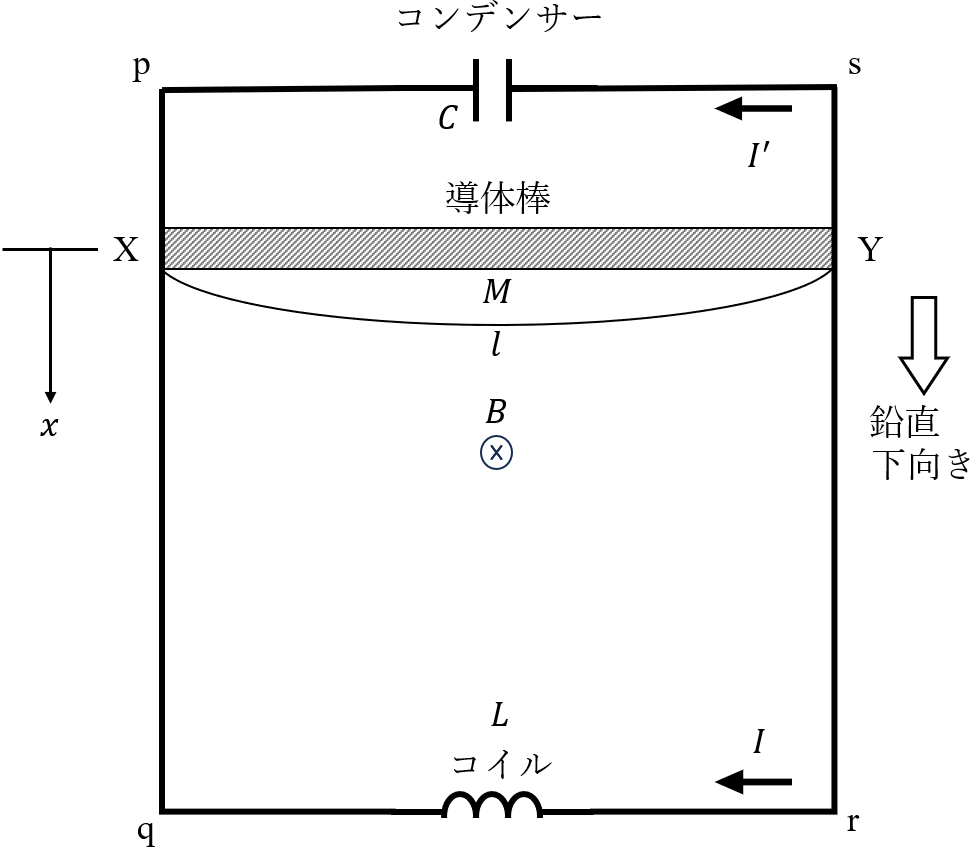
\includegraphics[width=.5\columnwidth]{../graphs/jumon_134.png}
  \caption{}
  \label{fig:j134}
\end{figure}



% メモ
\begin{comment}

\end{comment}


%%%%%%%%%%%%%%%%%%
